\section{Números aleatorios y semillas}

Bienvenido a la última parte de este texto. Siéntase orgulloso: después de haber dominado temas que le darían pesadillas a un matemático medieval, llegamos a algo más sencillo.

\subsection{Números aleatorios}

Aunque Python trae su propia librería random, la versión de NumPy es mucho más potente porque está diseñada para trabajar con arreglos gigantes de un solo golpe y con una eficiencia envidiable.
\begin{verbatim}
    np.random()
\end{verbatim}


\subsubsection{Generar numeros aleatorios entre 0 y 1}

Esta función es el estándar para generar "probabilidades". Devuelve valores en un intervalo semiabierto \([0,1)\), lo que significa que puede salir 0, pero nunca llegará a ser exactamente 1.
\begin{verbatim}
    np.random.rand()
\end{verbatim}

Vealo con un ejemplo
\begin{pycode}{Número entre 0 y 1}
    import numpy as np

    print("Número aleatorio [0,1):", np.random.rand())
\end{pycode}

\subsubsection{Array de números aleatorios}

Si usted quisiera generar un array con números aleatorios utilice la función:
\begin{verbatim}
    np.random.rand()
\end{verbatim}

En código:
\begin{pycode}{Array aleatorio}
    import numpy as np

    print("Array 1D:", np.random.rand(5)) # 5 números aleatorios
    print("Matriz 2D:\n", np.random.rand(2, 3)) # Matriz 2x3
\end{pycode}

\subsubsection{Enteros aleatorios}

Esta función es la que usted usará cuando quiera simular el lanzamiento de un dado o elegir un ID de usuario al azar. Su estructura es muy clara:
\begin{verbatim}
    np.random.randint(inicio, fin (no lo incluye), cantidad)
\end{verbatim}

En código:
\begin{pycode}{Enteros aleatorios}
    import numpy as np
    
    print("Enteros aleatorios:", np.random.randint(1, 10, size=5))
    # 5 números entre 1 y 9
\end{pycode}


\subsection{Fijar semillas \textit{np.random.seed()}}

Las computadoras, por muy inteligentes que parezcan, son máquinas deterministas: no son realmente capaces de crear azar de la nada. Lo que hacen es ejecutar una fórmula matemática tan compleja que genera una lista de números que parecen aleatorios. A esto lo llamamos números \textit{pseudoaleatorios}.

La semilla (\textit{seed}) es el número inicial que se le entrega a esa fórmula. Si usted usa la misma semilla, la fórmula siempre arrancará en el mismo lugar y, por lo tanto, toda la secuencia de números siguientes será exactamente igual.

Pero ¿Cómo funciona? Imagine que tiene un libro gigante con mil millones de números escritos.
\begin{itemize}
\item \textbf{Sin semilla:} \textit{Python} abre el libro en una página cualquiera (basándose usualmente en el reloj interno de su computadora). Cada vez que corre el programa, el libro se abre en un lugar distinto.
\item \textbf{Con semilla \textit{np.random.seed(42)}:} Usted le ordena a \textit{Python}: "Abra siempre el libro en la página 42". No importa cuántas veces reinicie su computadora, la secuencia de números empezará siempre en el mismo renglón.
\end{itemize}

Véalo usted mismo: si corre este código, obtendrá los mismos decimales que yo:
\begin{pycode}{Efecto de la semilla}
import numpy as np

# Ponemos una semilla cualquiera (ej: 42)
np.random.seed(42)
print("Primer intento:", np.random.rand(3)) # [0.37454012, 0.95071431, 0.73199394]

#Si volvemos a poner la misma semilla...
np.random.seed(42)
print("Segundo intento:", np.random.rand(3)) # [0.37454012, 0.95071431, 0.73199394]
# Los resultados seran IDENTICOS.
\end{pycode}

¿Para qué nos sirve? En el análisis de datos, la aleatoriedad es necesaria pero peligrosa. Aquí es donde la semilla nos salva:
\begin{enumerate}
\item \textit{Reproducibilidad (La clave de la ciencia):} Si usted descubre una tendencia increíble en una simulación financiera, necesita que su jefe o su profesor puedan correr su código y ver exactamente lo mismo que vio usted. Sin la semilla, ellos obtendrían otros números y pensarían que usted se inventó las conclusiones.
\item \textit{Caza de errores (\textit{Debugging}):} Si su programa falla solo una de cada diez veces que genera datos al azar, arreglarlo es una pesadilla porque el error "desaparece" al reiniciar. Al fijar la semilla, el error se vuelve estable y usted puede diseccionarlo con calma.
\item \textit{Comparación justa:} Si quiere saber qué estrategia de inversión es mejor, debe probar ambas bajo las mismas crisis y bonanzas. La semilla le permite crear un escenario "al azar" idéntico para todos sus modelos.
\end{enumerate}



\subsection{Distribuciones comunes estadísticas}

En el análisis de datos, las distribuciones son modelos matemáticos que describen con qué frecuencia ocurre cada valor en un conjunto de datos. No todos los datos se comportan igual: algunos prefieren amontonarse en el centro y otros se reparten democráticamente.

\subsubsection{Distribucion Uniforme}

Es aquella en la que todos los resultados posibles tienen exactamente la misma probabilidad de ocurrir. Visualmente, en un histograma, se ve como un rectángulo perfectamente plano. No hay "campana" ni picos; es una meseta de probabilidad donde el azar no tiene favoritos. Vease la figura \ref{distribución_uniforme_numpy}

Dependiendo de si necesita números enteros o decimales, \textit{NumPy} le ofrece tres herramientas principales:

\begin{enumerate}
\item \textit{Uniforme Continua (\texttt{np.random.rand} o \texttt{np.random.uniform}):} Genera números decimales. Se usa cuando el dato puede tener infinitos valores intermedios, como el tiempo exacto de espera de un buque en el puerto o la tasa de interés diaria de un bono.
\item \textit{Uniforme Discreta (\texttt{np.random.randint}):} Genera números enteros. Se usa cuando el dato es contable, como elegir un contenedor al azar de un lote de 100 o simular el número de una factura.
\end{enumerate}


\begin{figure}[!ht]
\centering
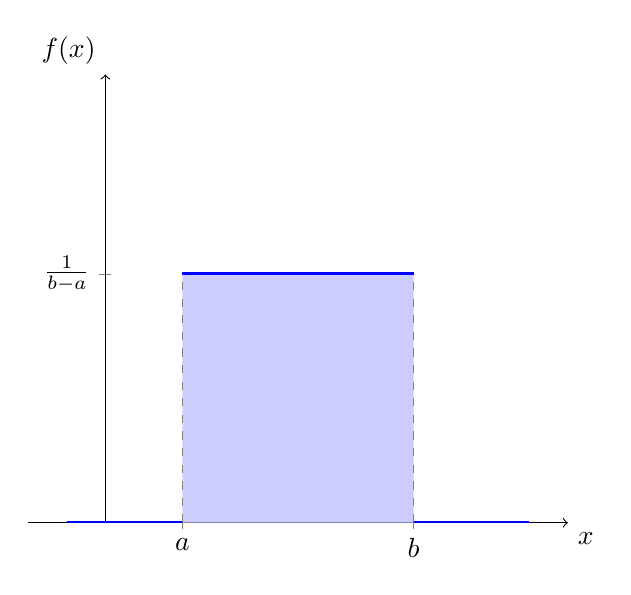
\begin{tikzpicture}
  \begin{axis}[
    axis lines = middle,
    xlabel = {$x$},
    ylabel = {$f(x)$},
    ymin = 0, ymax = 0.6,
    xmin = -1, xmax = 6,
    xtick = {1, 4},
    xticklabels = {$a$, $b$},
    ytick = {0.333},
    yticklabels = {$\frac{1}{b-a}$},
    every axis x label/.style={at={(current axis.right of origin)},anchor=north west},
    every axis y label/.style={at={(current axis.above origin)},anchor=south east},
    axis line style={->},
  ]

  % Área sombreada bajo la curva
  \addplot [fill=blue!20, draw=none, domain=1:4] {1/3} \closedcycle;

  % Líneas de la distribución uniforme
  \addplot [very thick, blue, domain=1:4] {1/3};
  
  % Líneas verticales discontinuas para los límites a y b
  \draw [dashed, gray] (axis cs:1,0) -- (axis cs:1,0.333);
  \draw [dashed, gray] (axis cs:4,0) -- (axis cs:4,0.333);

  % Líneas en cero para x < a y x > b
  \addplot [very thick, blue, domain=-0.5:1] {0};
  \addplot [very thick, blue, domain=4:5.5] {0};

  \end{axis}
\end{tikzpicture}
\caption{Representación de una distribución uniforme}
\label{distribución_uniforme_numpy}
\end{figure}

\paragraph{¿Para qué sirve en la vida real?}
\begin{itemize}
\item \textbf{Sorteos y Muestreos:} Si quiere auditar 10 documentos de un total de 500, usa esta distribución para asegurar que el documento 1 tenga la misma chance de ser revisado que el 500.
\item \textbf{Simulaciones Iniciales:} Cuando no tiene idea de cómo se comporta una variable (por ejemplo, el precio de un nuevo \textit{commodity}), empieza asumiendo que puede valer cualquier cosa entre un mínimo y un máximo con la misma probabilidad.
\item \textbf{Criptografía:} Las claves de seguridad se generan buscando una distribución uniforme perfecta para que un atacante no pueda predecir qué números salen más seguido.
\end{itemize}

Veamos una distribucion uniforme en código:
\begin{pycode}{Distribucion Uniforme}

import numpy as np

# 1. Decimales entre 0 y 1 (5 valores)
decimales = np.random.rand(5)

# 2. Decimales en un rango especifico (ej: entre 10 y 50)
precios_azar = np.random.uniform(10, 50, size=5)

# 3. Enteros (Simular el lanzamiento de un dado 10 veces)
dados = np.random.randint(1, 7, size=10) # El limite superior (7) no se incluye
\end{pycode}




\subsubsection{Distribución normal o Gausseana}

Aquí los datos tienen un favorito: el promedio. Es la forma que toman casi todos los fenómenos naturales y sociales cuando tienes una muestra lo suficientemente grande. En NumPy, la generamos principalmente con \texttt{np.random.randn()} o \texttt{np.random.normal()}.

Se la conoce como la Campana de Gauss. Su característica principal es la simetría. La mayoría de los datos se concentran en el centro (donde están la media, la mediana y la moda), a medida que te alejas del centro hacia la izquierda o derecha, la frecuencia de los datos cae rápidamente. Los valores "extremos" (muy altos o muy bajos) son muy poco probables. Vea la figura \ref{distribución_gausseana_numpy}.

\pgfmathdeclarefunction{gauss}{3}{%
  \pgfmathparse{1/(#3*sqrt(2*pi))*exp(-((#1-#2)^2)/(2*#3^2))}%
}
\begin{figure}[!ht]
    \centering
    \begin{tikzpicture}
  \begin{axis}[
    no markers, 
    domain=-4:4, 
    samples=100,
    axis lines=left, 
    xlabel=$x$, ylabel=$f(x)$,
    every axis y label/.style={at=(current axis.above origin),anchor=south},
    every axis x label/.style={at=(current axis.right of origin),anchor=west},
    height=5cm, width=10cm,
    xtick={-3, -2, -1, 0, 1, 2, 3},
    ytick=\empty,
    enlargelimits=false, 
    clip=false, 
    axis on top,
    grid = none
  ]

  % Área bajo la curva (68% - Una desviación estándar)
  \addplot [fill=blue!20, draw=none, domain=-1:1] {gauss(x, 0, 1)} \closedcycle;

  % Curva de la distribución normal
  \addplot [very thick, cyan!50!black] {gauss(x, 0, 1)};

  % Etiquetas de parámetros
  \draw [dashed] (axis cs:0,0) -- (axis cs:0,{gauss(0,0,1)}) 
    node[above] {$\mu$};
    
  % Indicación de Sigma
  \draw [latex-latex] (axis cs:0, 0.2) -- (axis cs:1, 0.2) 
    node[midway, above] {$\sigma$};

  \end{axis}
\end{tikzpicture}
\caption{Distribución normal o gausseana}
\label{distribución_gausseana_numpy}
\end{figure}

La distribución normal tiene dos numeros importantes:
\begin{itemize}
    \item La media(\(\mu\)): Indica donde esta el centro o promedio de la campana.
    \item La desviación estandar (\(\omega\)): Indica que tan ancha o flaca es la campana. Si la desviación es pequeña todos los datos se encuentran pegados al promedio, si es grande los datos estan más dispersos.
\end{itemize}

En análisis de datos, usamos la distribución normal porque nos permite predecir el futuro con márgenes de error:
\begin{itemize}
    \item Control de Calidad: Si una máquina llena botellas de 500ml, el llenado real seguirá una distribución normal. Si una botella sale con 450ml, sabemos que es un "error extraño" porque está muy lejos del centro de la campana.
    \item Finanzas y Riesgo: Los rendimientos de las acciones suelen modelarse así. La desviación estándar nos dice qué tan arriesgada es una inversión.
    \item Biometría y Sociología: La altura de las personas, los coeficientes intelectuales o los errores de medición en experimentos científicos.
\end{itemize}

Veamos como se realiza la campana de gauss en \textit{NumPy}
\begin{pycode}{Distribucion Normal}
import numpy as np

# 1. Normal Estandar (Media = 0, Desviacion = 1)
datos_estandar = np.random.randn(1000) # Generamos 1000 puntos para que se note la forma

# 2. Normal Personalizada (Media, Desviacion, Cantidad)
alturas = np.random.normal(175, 10, 1000) # Altura promedio 175cm con dispersion de 10cm

# 3. Ver el promedio real de los datos generados
print(f"Media real: {np.mean(alturas)}") # Deberia ser muy cercano a 175
\end{pycode}




\subsubsection{Distribución binomial}

Es la que usamos cuando los datos no son medidas (como la altura o el peso), sino conteos de éxitos o fracasos. Es la distribución del "Sí o No", del "Pasa o no Pasa". En NumPy, la generamos con \texttt{np.random.binomial()}.

Imagina que realizas un experimento (como lanzar una moneda) un número determinado de veces (\(n\)). En cada intento, solo hay dos resultados posibles: Éxito o Fracaso. La distribución binomial te dice cuál es la probabilidad de obtener exactamente \(k\) éxitos en esos n intentos, conociendo de antemano la probabilidad \(p\) de que un solo intento sea exitoso.


Para que NumPy calcule esta distribución, necesita tres parámetros:
\begin{itemize}
    \item \textit{n (n)}: El número de veces que repites el experimento (ej: lanzas la moneda 10 veces).
    \item \textit{p (prob)}: La probabilidad de éxito en un solo intento (ej: 0.5 para una moneda, o 0.05 para una pieza fallada).
    \item \textit{size}: Cuántas veces quieres repetir todo el conjunto de experimentos para ver los resultados.
\end{itemize}
    
¿Para qué sirve?  En comercio y control de procesos, es la herramienta fundamental para la toma de decisiones, ya que permite:
\begin{itemize}
    \item Control de Calidad: Si sabes que el \(2\%\) de las piezas de una fábrica suelen salir falladas, la distribución binomial te dice qué tan probable es que en un lote de 100 piezas encuentres más de 5 falladas (lo cual indicaría que algo anda mal en la máquina).
    \item Conversión de Ventas: Si un vendedor tiene una tasa de cierre del \(10\%\), ¿cuál es la probabilidad de que logre 3 ventas si llama a 20 clientes hoy?
    \item Logística: Si la probabilidad de que un camión se retrase en la frontera es del \(15\%\), ¿cuántos camiones de una flota de 10 llegarán tarde probablemente?
\end{itemize}
    

En \textit{NumPy }esto se ve así:
\begin{pycode}{Distribucion Binomial}
import numpy as np

# Ejemplo: Lanzamos una moneda 10 veces (n=10)
# La probabilidad de cara es 0.5 (p=0.5)
# Queremos simular este juego 1 vez
exitos = np.random.binomial(n=10, p=0.5, size=1) 
print(f"Caras obtenidas: {exitos}")

# Ejemplo de Negocios:
# Probabilidad de que un cliente pague a término: 0.8 (p)
# Tenemos 100 clientes (n)
# Simulamos 1000 meses para ver el comportamiento (size)
pagos_a_termino = np.random.binomial(n=100, p=0.8, size=1000)

print(f"Promedio de clientes que pagan a término: {np.mean(pagos_a_termino)}")
\end{pycode}